\documentclass[12pt,oneside,a4paper]{article}
\usepackage{graphicx}
\usepackage{hyperref}
\usepackage[utf8]{inputenc}
\usepackage[english, czech]{babel}
\usepackage{listings}

\usepackage{xcolor} % Required for specifying custom colors
\usepackage{fix-cm} % Allows increasing the font size of specific fonts beyond LaTeX default specifications

\setlength{\oddsidemargin}{0mm} % Adjust margins to center the colored title box
\setlength{\evensidemargin}{0mm} % Margins on even pages - only necessary if adding more content to this template

\newcommand{\HRule}[1]{\hfill \rule{0.2\linewidth}{#1}} % Horizontal rule at the bottom of the page, adjust width here

\definecolor{grey}{rgb}{0.9,0.9,0.9} % Color of the box surrounding the title - these values can be changed to give the box a different color	


\begin{document}

\thispagestyle{empty} % Remove page numbering on this page

%----------------------------------------------------------------------------------------
%	TITLE SECTION
%----------------------------------------------------------------------------------------

\colorbox{grey}{
	\parbox[t]{1.0\linewidth}{
		\centering \fontsize{30pt}{50pt}\selectfont % The first argument for fontsize is the font size of the text and the second is the line spacing - you may need to play with these for your particular title
		\vspace*{0.7cm} % Space between the start of the title and the top of the grey box
		
		\hfill 1. Term Paper (CP1) \\
		\hfill Databázové systémy \\
		\hfill A4B33DS\par
		
		\vspace*{0.7cm} % Space between the end of the title and the bottom of the grey box
	}
}

%----------------------------------------------------------------------------------------

\vfill % Space between the title box and author information

%----------------------------------------------------------------------------------------
%	AUTHOR NAME AND INFORMATION SECTION
%----------------------------------------------------------------------------------------

{\centering \large 
\hfill Martin Indra \\
\hfill Czech Technical University in Prague \\
\hfill \texttt{indrama1@fel.cvut.cz} \\

\HRule{1pt}} % Horizontal line, thickness changed here

%----------------------------------------------------------------------------------------

\clearpage % Whitespace to the end of the page
\newpage

\section{Logical Modeling}

User is a single person and this person can use multiple devices, overmore some devices can be represented by multiple unique indetificators (for instance phone number). That's why there is table ``collabms\_{}identificator'' which represents one indentificator and every user has zero or more identificators (relation 1:0..N).

Every user can have messages targeting him and each message can be received to one or more users. This relation (M:N) is provided by ``collabms\_{}has\_{}message'' table. Messages have authors therefore message linking to user (relation 1:1).

Hence users are able to invite others to painting room, there is ``collabms\_{}invitation'' table. Message can contain invitation so that message may link to invitation (0..1:1 relation). The table linking to ``collabms\_{}server'' (relation 1:1) because this table represents invitation to room on some  \emph{server}.

The table ``collabms\_{}user\_{}has\_{}room\_{}shot'' provide M:N relation between users and room shots. Room shot is a save of room or its screenshot.

\begin{figure}[h]
	\centering
	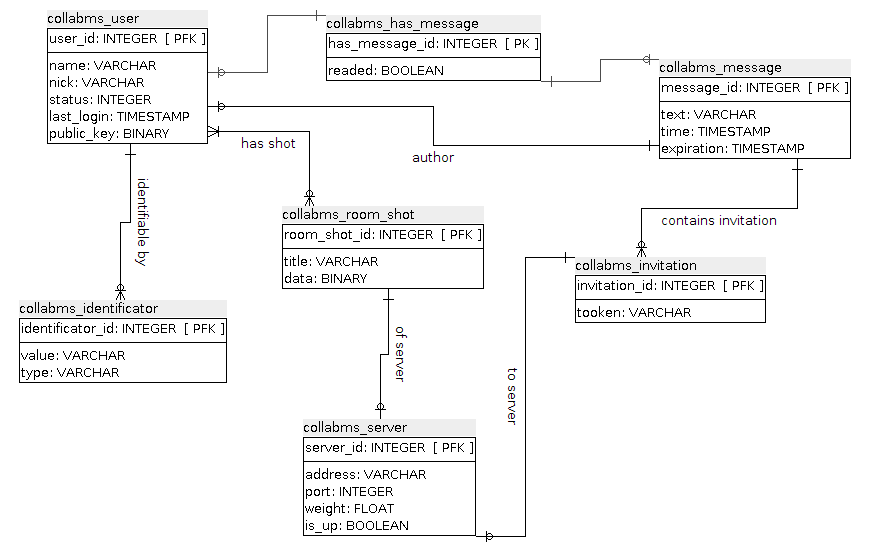
\includegraphics[width=0.9\textwidth]{figures/logical_model.png}
	\caption{Logical Modeling}
	\label{fig.logical_model}
\end{figure}

\section{SQL Script Creating Database}

\lstinputlisting[language=SQL]{create.sql}
\newpage

\section{Commented Referential Integrity}

\noindent
Table collabms\_has\_message is weak refferential type. If we delete user or message from database him messages should be deleted too.

\begin{lstlisting}[language=SQL]
ALTER TABLE collabms_has_message ADD CONSTRAINT user_id
FOREIGN KEY (user_id) REFERENCES collabms_user (user_id)
ON DELETE CASCADE ON UPDATE CASCADE;
\end{lstlisting}

\begin{lstlisting}[language=SQL]
ALTER TABLE collabms_has_message ADD CONSTRAINT message_id
FOREIGN KEY (user_id) REFERENCES collabms_user (user_id)
ON DELETE CASCADE ON UPDATE CASCADE;
\end{lstlisting}

\noindent
Message should not be deleted after deleting user because it will be still useful for recipients.

\begin{lstlisting}[language=SQL]
ALTER TABLE collabms_message ADD CONSTRAINT author
FOREIGN KEY (author) REFERENCES collabms_user (user_id)
ON DELETE SET NULL UPDATE CASCADE;
\end{lstlisting}

\noindent
Message should not be deleted after deleting invitation because it can be still useful for recipients (containing aditional message).

\begin{lstlisting}[language=SQL]
ALTER TABLE collabms_message ADD CONSTRAINT invitation
FOREIGN KEY (invitation) REFERENCES collabms_invitation (invitation_id)
ON DELETE SET NULL UPDATE CASCADE;
\end{lstlisting}

\noindent
Delete user's room shots after deleting room shot or user.

\begin{lstlisting}[language=SQL]
ALTER TABLE collabms_user_has_room_shot ADD CONSTRAINT user_id
FOREIGN KEY (user_id) REFERENCES collabms_user (user_id)
ON DELETE CASCADE ON UPDATE CASCADE;
\end{lstlisting}

\begin{lstlisting}[language=SQL]
ALTER TABLE collabms_user_has_room_shot ADD CONSTRAINT room_shot
FOREIGN KEY (room_shot) REFERENCES collabms_room_shot (room_shot_id)
ON DELETE CASCADE ON UPDATE CASCADE;
\end{lstlisting}

\noindent
Room shot can be still userful after server deletion.

\begin{lstlisting}[language=SQL]
ALTER TABLE collabms_room_shot ADD CONSTRAINT server
FOREIGN KEY (server) REFERENCES collabms_server (server_id)
ON DELETE SET NULL ON UPDATE CASCADE;
\end{lstlisting}

\noindent
Identificator should be removed after deletion of user because it identificates just him.

\begin{lstlisting}[language=SQL]
ALTER TABLE collabms_identificator ADD CONSTRAINT user_id
FOREIGN KEY (user_id) REFERENCES collabms_user (user_id)
ON DELETE CASCADE ON UPDATE CASCADE;
\end{lstlisting}

\begin{lstlisting}[language=SQL]

\end{lstlisting}

\end{document}
